\section{Resultados esperados}

Como resultado final desse trabalho, espera-se o desenvolvimento de um protocolo para controle de acesso ao meio (\textit{MAC protocol}) auto-organizado capaz de aumentar a eficiência da rede em termos de latência e economia de energia. 

O protocolo desenvolvido deverá ser capaz de produzir uma organização na rede de sensores de tal forma que seja criada uma sub-estrutura(composta por uma parte dos nós selecionados por um processo de eleição) onde os nós participantes serão sincronizados com uma pequena variação de acordo com o tempo necessário para transmissão de uma mensagem entre dois nós subsequentes. 

Supondo que os nós A, B, C e D façam parte dessa subestrutura, eles seriam sincronizados com um pequeno atraso entre eles, de forma que, na transmissão de uma mensagem de A para D passando por B e C, o tempo de transmissão entre A e B seja menor que o tempo que C leva para acordar depois que A acorda. Espera-se com isso conseguir que o tempo de espera para transmissão de mensagem de cada nó dessa subestrutura seja mínimo. 

Fora dessa subestrutura, a transmissão de mensagens e os ciclos de sono serão controlados por outros protocolos já existentes Considerando que a transmissão de mensagens aconteça entre nós distantes, espera-se que tempo médio de transmissão na rede como um todo também seja reduzido, uma vez que os atrasos causados por tempo de espera para transmissão só ocorram até que mensagem chegue a um nó que pertença à subestrutura formada. 

Como produtos desse trabalho devem ser desenvolvidos:
 
 \subsubsection{Algoritmo de eleição:} esse algoritmo deverá selecionar os melhores candidatos a fazer parte da estrutura com base em seus atributos, por exemplo capacidade de transmissão ou nível de carga da bateria, etc.
 
 \subsubsection{Algoritmo para sincronização:} o algoritmo deverá ser capaz de sincronizar os ciclos de sono dos nós eleitos de forma a porssibilitar a apresentação das características descritas anteriormente.
 
 \subsubsection{Resultados de testes:} apresentação da análise de eficiência do algoritmo com base em simulações computacionais, bem como uma comparação com protocolos já existentes.
 
 \section{Cronograma}
 
\begin{figure}[!htb]
\centering
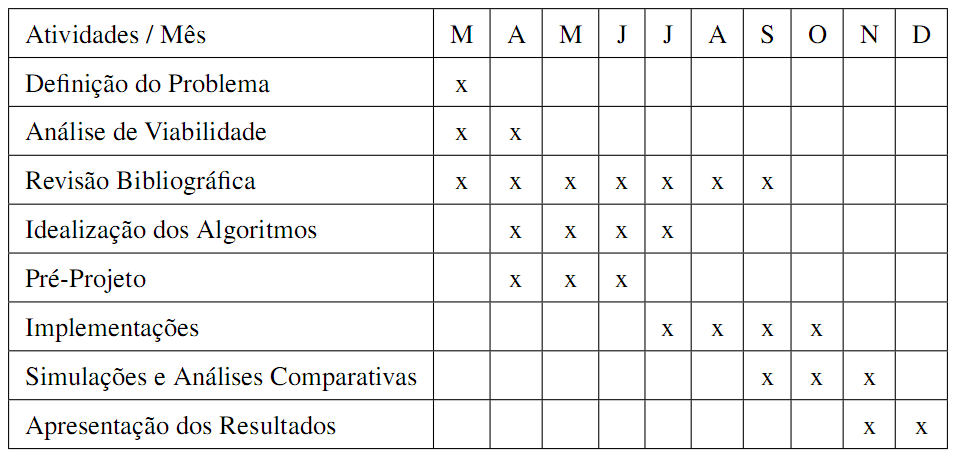
\includegraphics[width=400px,height=180px]{./Pictures/cronograma.png}
% SensorNodesScatteredInASensorField.png: 816x1056 pixel, 96dpi, 21.59x27.94 cm, bb=0 0 612 792
% pdfLaTeX aceita figuras no formato PNG, JPG ou PDF
% figuras vetoriais podem ser exportadas para eps e depois convertidas para pdf usando epstopdf
\caption{Cronograma para o desenvolvimento do projeto} %legenda
\label{fig:cronograma} %rotulo para refencia
\end{figure}